\section{Methods} \label{methods}

\subsection{Study population}
The paper will analyze data from the Hamburg City Health Study (HCHS), which is an ongoing prospective, population-based cohort study aiming to recruit a cross-sectional sample of \num{45000} adult participants from the city of Hamburg, Germany \citep{Jagodzinski2020-lx}.
From the first \num{10000} participants of the HCHS we will aim to include those who were documented to have received brain imaging (n=2652) and exclude those who were analyzed in our previous report \citep{Schlemm2022-he}.
The ethical review board of the Landesärztekammer Hamburg (State of Hamburg Chamber of Medical Practitioners) approved the HCHS (PV5131), all participants provided written informed consent.

\subsection{Demographic and clinical characterization}
From the study database we will extract participants’ age at the time of inclusion in years, their self-reported gender and the number of years spent in education.
During the visit at the study center, participants undergo cognitive assessment using standardized tests.
We will extract from the database their performance scores in the Trail Making Test part B, measured in seconds, as an operationalization of executive function and psychomotor processing speed \citep{Tombaugh2004-dp,arbuthnott2000trail}.

\subsection{MRI acquisition and preprocessing}
The magnetic resonance imaging protocol for the HCHS includes structural and resting-state functional sequences.
The acquisition parameters on a \qty{3}{\tesla} Siemens Skyra MRI scanner (Siemens, Erlangen, Germany) have been reported before \citep{Petersen2020-cx,Frey2021-sv} and are given as follows:

For $T_1$-weighted anatomical images, a 3D rapid acquisition gradient-echo sequence (MPRAGE) was used with the following sequence parameters: repetition time $\text{TR} = \qty{2500}{\ms}$, echo time $\text{TE} = \qty{2.12}{\ms}$, 256 axial slices, slice thickness $\text{ST} = \qty{0.94}{\mm}$, and in-plane resolution  $\text{IPR} = \qtyproduct[product-units = bracket-power]{0.83 x 0.83}{\mm}$.

$T_2$-weighted fluid attenuated inversion recovery (FLAIR) images were acquired with the following sequence parameters: $\text{TR} = \qty{4700}{\ms}$, $\text{TE} = \qty{392}{\ms}$, \num{192} axial slices, $\text{ST} = \qty{0.9}{\mm}$, $\text{IPR} = \qtyproduct[product-units = bracket-power]{0.75 x 0.75}{\mm}$.

\num{125} resting state functional MRI volumes were acquired ($\text{TR} = \qty{2500}{\ms}$; $\text{TE} = \qty{25}{\ms}$; $\text{flip angle} = \ang[]{90}$; slices = \num{49}; $\text{ST} = \qty{3}{\mm}$; $\text{slice gap} = \qty{0}{\mm}$; $\text{IPR} = \qtyproduct[product-units = bracket-power]{2.66 x 2.66}{\mm}$).
Subjects were asked to keep their eyes open and to think of nothing.

We will verify the presence and voxel-dimensions of expected MRI data for each participant and exclude those for whom at least one of $T_1$-weighted, FLAIR and resting-state MRI is missing. We will also exclude participants with a neuroradiologically confirmed space-occupying intra-axial lesion.
To ensure reproducibility, no visual quality assessment on raw images will be performed.

For the remaining participants, structural and resting-state functional MRI data will be preprocessed using FreeSurfer v6.0 (\url{https://surfer.nmr.mgh.harvard.edu/}), and fmriPrep v20.2.6 \citep{Esteban2019-sx}, using default parameters. Participants will be excluded if automated processing using at least one of these packages fails.

\subsection{Quantification of WMH load}
For our primary analysis, the extent of ischemic white matter disease will be operationalized as the total volume of supratentorial WMHs obtained from automated segmentation using a combination of anatomical priors, BIANCA \citep{Griffanti2016-dt} and LOCATE \citep{Sundaresan2019-ww}, post-processed with a minimum cluster size of \num{30} voxels, as described in \citep{Schlemm2022-he}.
In an exploratory analysis, we partition voxels identified as WMH into deep and periventricular components according to their distance to the ventricular system (cut-off $\qty{10}{\mm}$, \citep{Griffanti2018-oa})

\subsection{Brain state estimation}
Output from fMRIprep will be post-processed using xcpEngine v1.2.1 to obtain de-confounded spatially averaged BOLD time series \citep{Ciric2017-cl}.
For the primary analysis we will use the \textit{36p} regression strategy and the Schaefer-\num{400} parcellation \citep{Schaefer2018-bo}, as in \citep{Schlemm2022-he}.
 
Different atlases and confound regression strategies, as implemented in xcpEngine, will be included in the exploratory multiverse analysis.

Co-activation pattern (CAP) analysis will be performed by first aggregating parcellated, de-confounded BOLD signals into a $\left(n_{\text{parcels}}\times \sum_i{n_{\text{time points}, i}}\right)$ feature matrix, where $n_{\text{time points}, i}$ denotes the number of retained volumes for subject $i$ after confound regression.
Clustering will be performed using the $k$-means algorithm ($k=5$) with distance measure given by 1 minus the sample Pearson correlation between points, as implemented in Matlab R2021a.
We will estimate subject- and state-specific fractional occupancies, which are defined as the proportion of BOLD volumes assigned to each brain state \citep{Vidaurre2018-pb}. 
The two states with the highest average occupancy will be identified as the basis for further analysis.


\subsection{Statistical analysis}
For demographic (age, gender, years of education) and clinical (TMT-B) variables the number of missing records will be reported.
For non-missing values, we will provide descriptive summary statistics using median and interquartile range.
The proportion of men and women in the sample will be reported. Regression modelling will be carried out as a complete-case analysis.

As a first outcome-neutral quality check of the implementation of the MRI processing pipeline, brain state estimation and co-activation pattern analysis, we will compare fractional occupancies between brain states.
We expect that the average fractional occupancy in two high-occupancy states is higher than the average fractional occupancy in the other three states.
Point estimates and 95\% confidence intervals will be presented for the difference in average fractional occupancy to check this assertion.

For further analyses, non-zero WMH volumes will be subjected to a logarithmic transformation.
Zero values will retain their value zero; to compensate, all models will include a binary indicator for zero WMH volume if at least one non-zero value is present.

To assess the primary hypothesis of a negative association between the extent of ischemic white matter disease and time spent in high-occupancy brain states, we will perform a fixed-dispersion beta-regression to model the logit of the conditional expectation of the average fractional occupancy of two high-occupancy states as an affine function of the logarithmized WMH load.
Age and gender will be included as covariates.
The strength of the association will be quantified as an odds ratio per interquartile ratio of the WMH burden distribution and accompanied by a 95\% confidence interval.
Significance testing of the null hypothesis of no association will be conducted at the conventional significance level of 0.05.
Estimation and testing will be carried out using the 'betareg' package v3.1.4 in R v4.2.1.

To  assess the secondary hypothesis of an association between time spent in high-occupancy brain states and executive dysfunction, we will perform a generalized linear regression with a Gamma response distribution to model the logarithm of the conditional expected completion time in part B of the TMT as an affine function of the average fractional occupancy of two high-occupancy states.
Age, gender, years of education and logarithmized WMH load will be included as covariates.
The strength of the association will be quantified as a multiplicative factor per percentage point and accompanied by a 95\% confidence interval.
Significance testing of the null hypothesis of no association will be conducted at the conventional significance level of 0.05.
Estimation and testing will be carried out using the glm function included in the 'stats' package from R v4.2.1.

Sample size calculation is based on an effect size on the odds ratio scale of 0.95, corresponding to an absolute difference in the probability of occupying a DMN-related brain state between the first and third WMH-load quartile of 1.3 percentage points, and between the 5\% and 95\% percentile of 3.1 percentage points. Approximating half the difference in fractional occupancy of DMN-related states between different task demands (rest vs n-back) in healthy subjects, which was estimated to lie between 6 and 7 percentage points \citep{Cornblath2020-fu}, this value represent a plausible choice for the smallest effect size of theoretical and practical interest. It also equals the effect size estimated based on the data presented in \citep{Schlemm2022-he}. 

We used simple bootstrapping to create \num{10000} hypothetical datasets of size \num{200}, \num{400}, \num{600}, \num{800}, \num{900}, \num{910}, \ldots, \num{1100}, \num{1200}, \num{1400}, \num{1500}, \num{1600}.
Each dataset was subjected to the estimation procedure described above.
For each sample size, the proportion of datasets in which the primary null hypothesis of no association between fractional occupancy and WMH load could be rejected at $\alpha=0.05$ was computed and is recorded as a power curve in \Cref{fig:power}.

\begin{figure}
    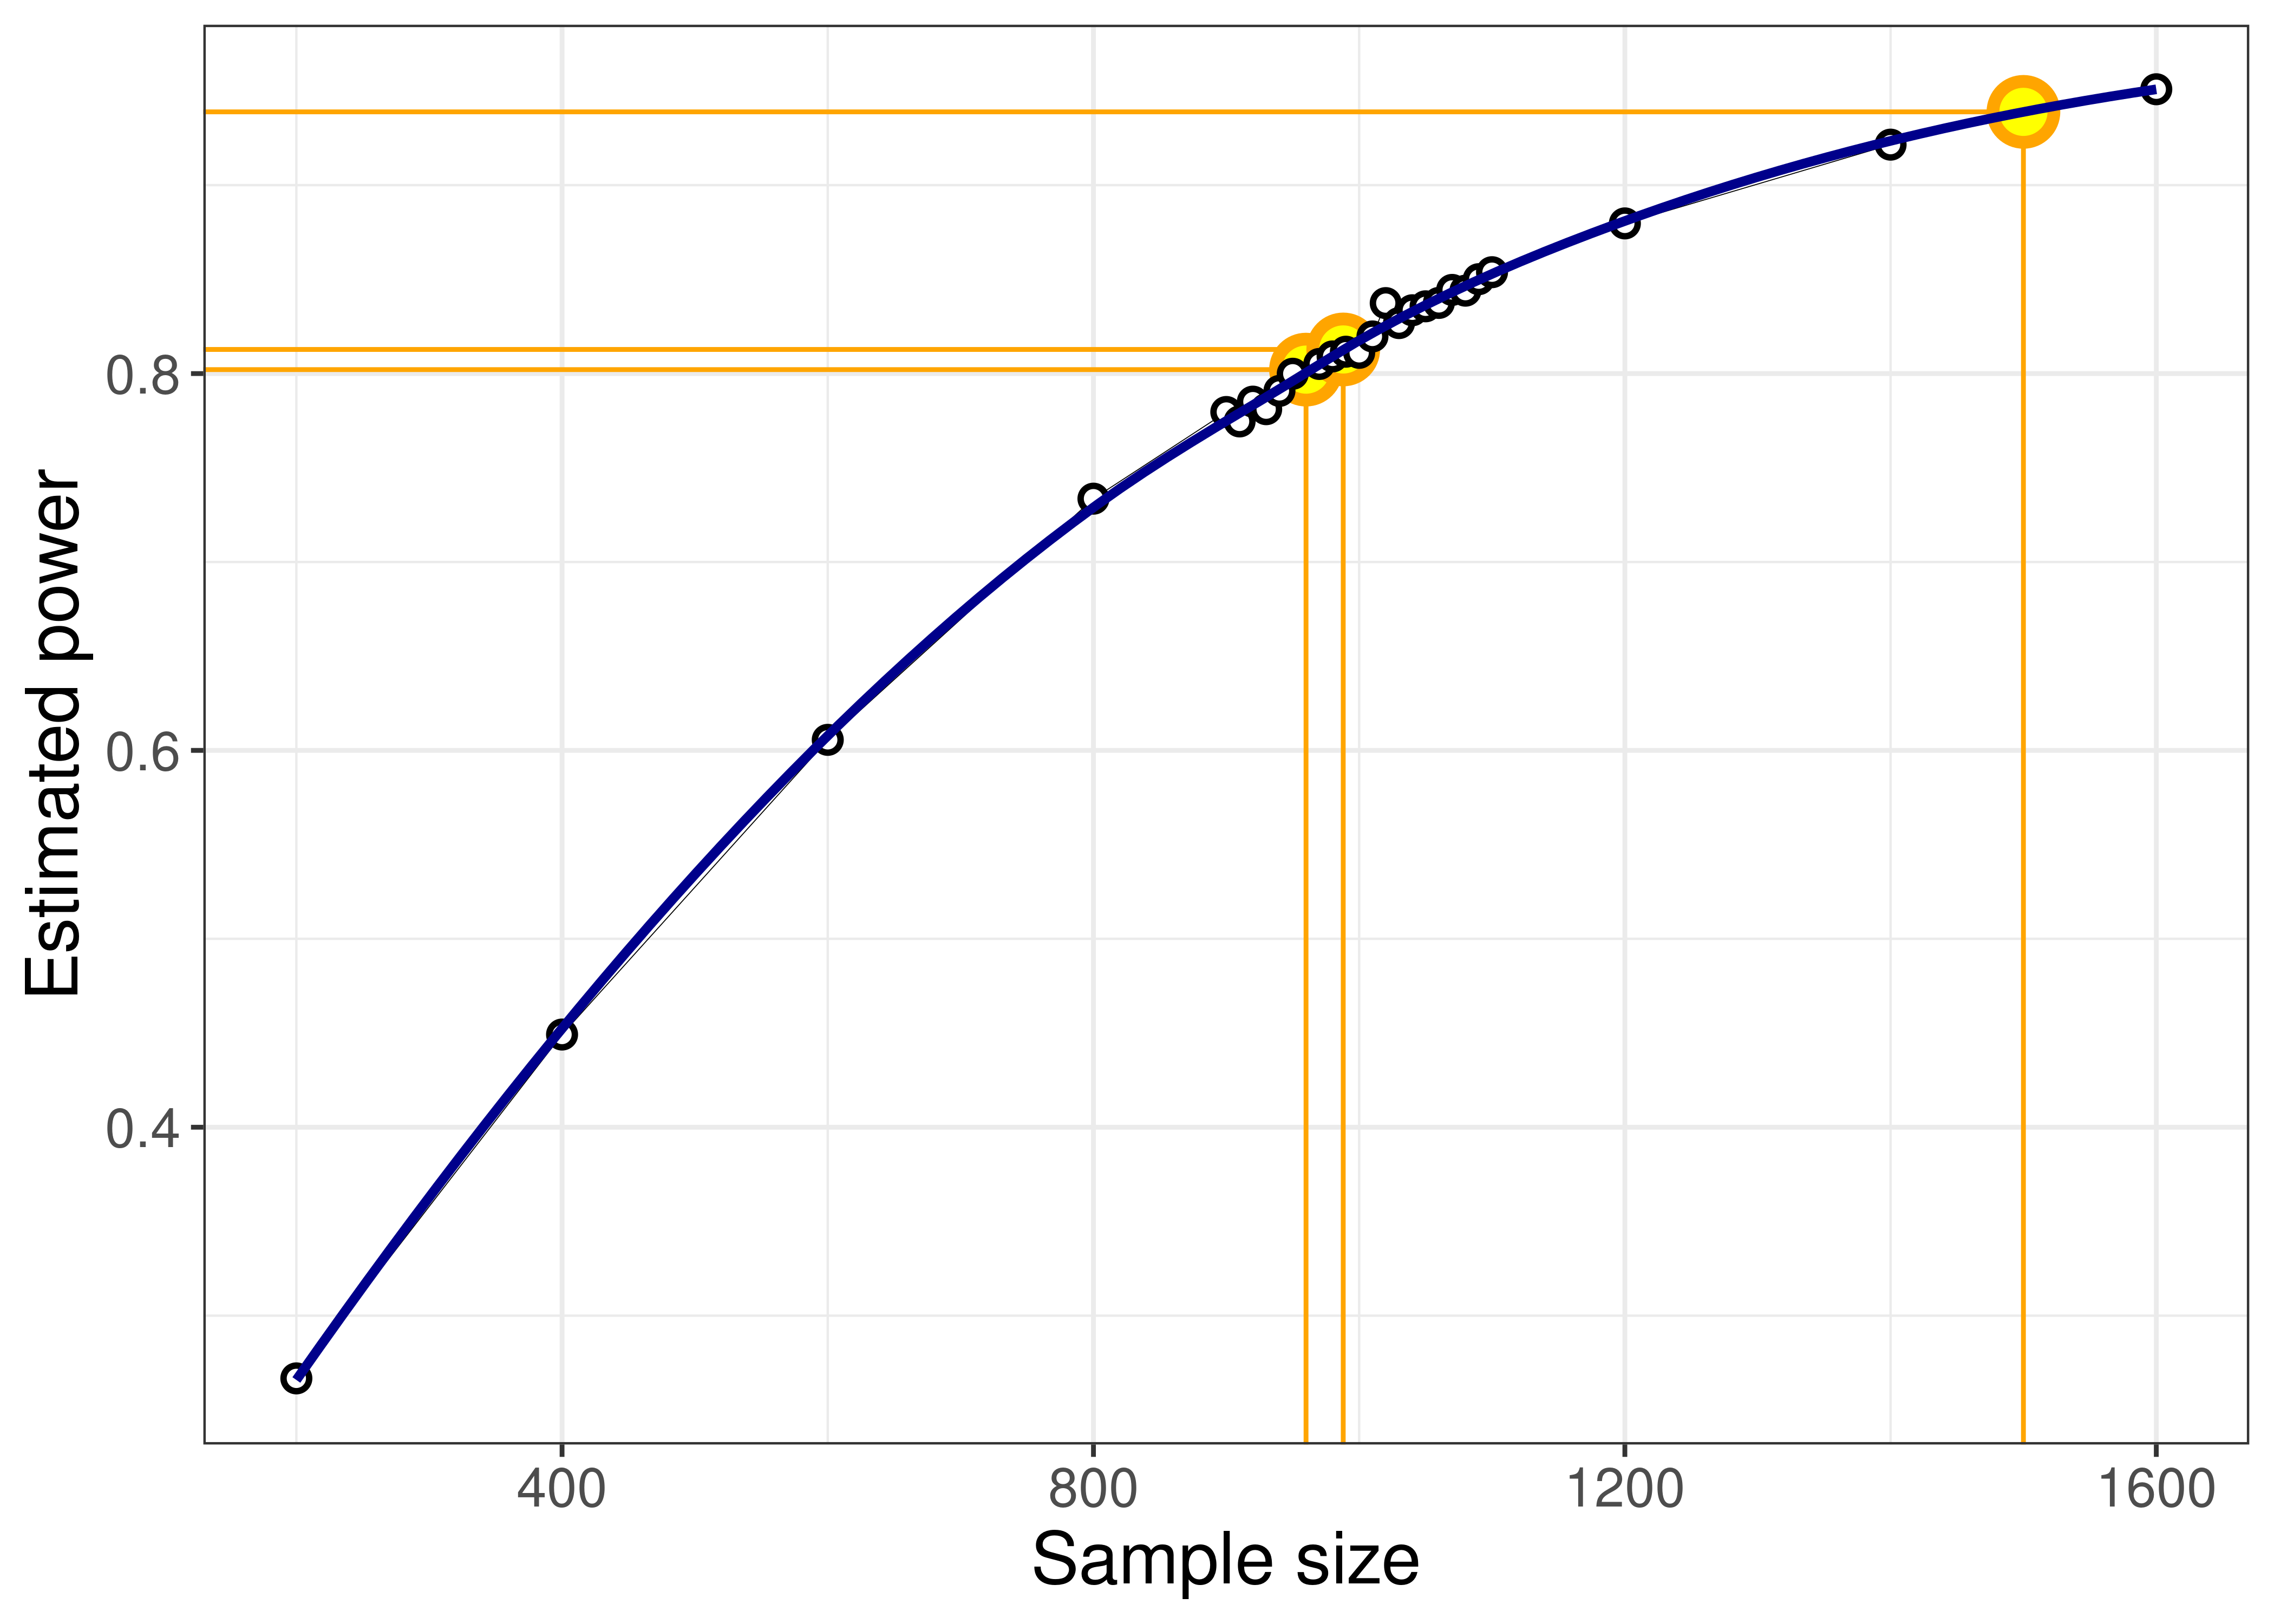
\includegraphics[width=.5\linewidth]{./../analysis/code/R/pipeline_files/figure-html/power-1.png}
    \caption{Estimated power for different sample sizes is obtained as the proportion of synthetic data sets in which the null hypothesis of no association between WMH volume and time spent in high-occupancy brain states an be rejected at the $\alpha=0.05$ significance level. Proportions are based on a total of \num{10000} synthetic data sets obtained by bootstrapping the data presented in \citep{Schlemm2022-he}. Highlighted in orange are the smallest sample size ensuring a power of at least \qty{80}{\percent} ($n=960$), the sample size of the pilot data ($n=988$, post-hoc power \qty{81.3}{\percent}), and the expected sample sample size for this replication study ($n=1500$, a-priori power \qty{93.9}{\percent}).}
    \label{fig:power}
\end{figure}

It is seen that a sample size of \num{960} would allow replication of the reported effect with a power of \qty{80.2}{\percent}.
We anticipate a sample size of \num{1500}, which yields a power of \qty{93.9}{\percent}.


\subsection{Multiverse analysis}
Both in \citep{Schlemm2022-he} and for our primary replication analysis we made certain analytical choices in the operationalization of brain states and ischemic white matter disease, namely the use of the \textit{36p} confound regression strategy, the Schaefer-\num{400} parcellation and a BIANCA/LOCATE-based WMH segmentation algorithm.
The robustness of the association between WMH burden and time spent in high-occupancy states with regard to other choices will be explored in a multiverse analysis \citep{Steegen2016-ze}. Specifically, in an exploratory analysis, we will estimate brain states from BOLD time series processed according to a variety of established confound regression strategies and aggregated over different cortical brain parcellations (\Cref{tab:multiverse}, \cite{ciric2018mitigating,Ciric2017-cl}). Extent of cSVD will additionally be quantified by the volume of deep and periventricular white matter hyperintensities.

\renewcommand\cellset{\renewcommand\arraystretch{0.5}%
    \setlength\extrarowheight{0pt}}
\begin{table}[bt]
    \begin{threeparttable}
        \begin{subtable}[t]{.75\textwidth}
            \label{tab:parcellations2}
            % Use "S" column identifier to align on decimal point 
            \begin{tabularx}{\textwidth}{l l l}
                \toprule
                \textbf{Name of the atlas}  & \textbf{\#parcels}                                  & \textbf{Reference}          \\
                \midrule
                Desikan--Killiany           & \num{86}                                            & \cite{desikan2006automated} \\
                AAL                         & \num{116}                                           & \cite{tzourio2002automated} \\
                Harvard--Oxford             & \num{112}                                           & \cite{makris2006decreased}  \\
                glasser360                  & \num{360}                                           & \cite{Glasser2016-ia}       \\
                gordon333                   & \num{333}                                           & \cite{Gordon2016-wy}        \\
                power264                    & \num{264}                                           & \cite{Power2011-xf}         \\
                schaefer\{N\}               & \makecell[lt]{\num{100} \\ \num{200}\\ \num{400}}   & \cite{Schaefer2018-bo}      \\
                \bottomrule
            \end{tabularx}
            \begin{tablenotes}
                \item{AAL:} Automatic Anatomical Labelling
            \end{tablenotes}
            \caption{Parcellations}
        \end{subtable}
        \qquad
        \begin{subtable}[t]{.75\textwidth}
            \label{tab:parcellations}
            % Use "S" column identifier to align on decimal point 
            \begin{tabularx}{\textwidth}{l l l}
                \toprule
                \textbf{Design}        & \textbf{Reference}                 \\
                \midrule
                24p                    & \cite{friston1996movement}         \\
                24p + GSR              & \cite{macey2004method}             \\
                36p              & \cite{satterthwaite2013improved}   \\
                36p + spike regression & \cite{cox1996afni}                 \\
                36p + despiking        & \cite{satterthwaite2013improved}   \\
                36p + scrubbing  & \cite{power2014methods}            \\
                aCompCor               & \cite{muschelli2014reduction}      \\
                tCompCor               & \cite{behzadi2007component}        \\
                AROMA                  & \cite{pruim2015ica}                \\
                \bottomrule
            \end{tabularx}
            \begin{tablenotes}
                \item GSR: Global signal regression, AROMA: Automatic Removal of Motion Artifacts
            \end{tablenotes}
            \caption{Confound regression strategies, adapted from \citep{Ciric2017-cl}}
        \end{subtable}
        \makeatletter\def\TPT@hsize{}\makeatletter
    \end{threeparttable}
    \mycaption{Multiverse analysis}{Overview over different brain parcellations and confound regression strategies implemented using xcpEngine \citep{ciric2018mitigating}. A total of $9\times 9=81$ analytical combinations were explored to assess the robustness of our results with respect to these processing choices.}
    \label{tab:multiverse}
\end{table}

For each combination of analytical choice of confound regression strategy, parcellation and subdivision of white matter lesion load ($9\times9\times3=243$ scenarios in total) we will quantify the association between WMH load and average time spent in high-occupancy brain states using odds ratio and \qty{95}{\percent} confidence intervals as described above.

No hypothesis testing and will be carried out in these multiverse analyses. They rather serve to inform about the robustness of the outcome of the test of the primary hypothesis.
Any substantial conclusions about the association between severity of cerebral small pathology and time spent in high-occupancy brain states, as stated in the Scientific Question in \Cref{tab:SDT}, will be drawn from the primary analysis using pre-specified methodological choices.

\section{Further exploratory analysis}
In previous work, two high-occupancy brain states were related to the default-mode network \citep{Cornblath2020-fu}.
We will further explore this relation by computing, for each individual brain state, the cosine similarity of the positive and negative activations of the cluster’s centroid with a set of a-priori defined functional ‘communities’ or networks \citep{Schaefer2018-bo,Yeo2011-qg}.
Results will be thus visualized as spider plots for the Schaefer, Gordon and Power atlases.

In further exploratory analyses we plan to describe the associations between brain state dynamics and other measures of cognitive ability, such as memory and language.